\documentclass[12pt,a4paper]{article}
\usepackage[margin=2.5cm]{geometry}
\usepackage{graphicx} % Required for inserting images
\usepackage{float}
\usepackage{subcaption}
\usepackage{booktabs}
\usepackage{tikz}
\usetikzlibrary{positioning}


\title{4B23: Optical Network Design}
\author{Joe Leacy}

\begin{document}

\maketitle

\section{Introduction}

\begin{figure}[H]
\centering
\begin{subfigure}[b]{0.45\textwidth}
\centering
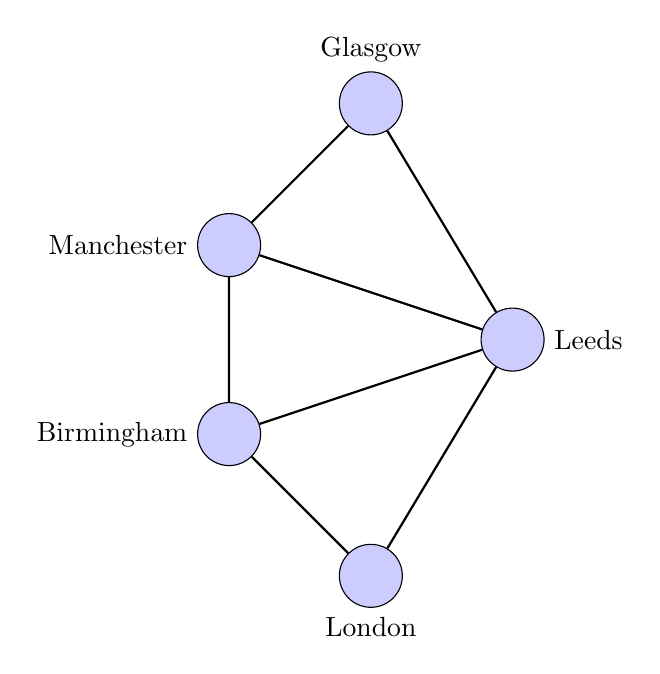
\begin{tikzpicture}[scale=1.2]
    % Define node positions (clockwise from bottom)
    \node[circle, draw, fill=blue!20, minimum size=0.8cm, label=below:London] (London) at (0, -2) {};
    \node[circle, draw, fill=blue!20, minimum size=0.8cm, label=left:Birmingham] (Birmingham) at (-1.5, -0.5) {};
    \node[circle, draw, fill=blue!20, minimum size=0.8cm, label=left:Manchester] (Manchester) at (-1.5, 1.5) {};
    \node[circle, draw, fill=blue!20, minimum size=0.8cm, label=above:Glasgow] (Glasgow) at (0, 3) {};
    \node[circle, draw, fill=blue!20, minimum size=0.8cm, label=right:Leeds] (Leeds) at (1.5, 0.5) {};
    
    % Draw edges
    \draw[thick] (London) -- (Birmingham);
    \draw[thick] (London) -- (Leeds);
    \draw[thick] (Birmingham) -- (Leeds);
    \draw[thick] (Birmingham) -- (Manchester);
    \draw[thick] (Manchester) -- (Leeds);
    \draw[thick] (Manchester) -- (Glasgow);
    \draw[thick] (Glasgow) -- (Leeds);
\end{tikzpicture}
\caption{Network 1}
\end{subfigure}
\hfill
\begin{subfigure}[b]{0.45\textwidth}
\centering
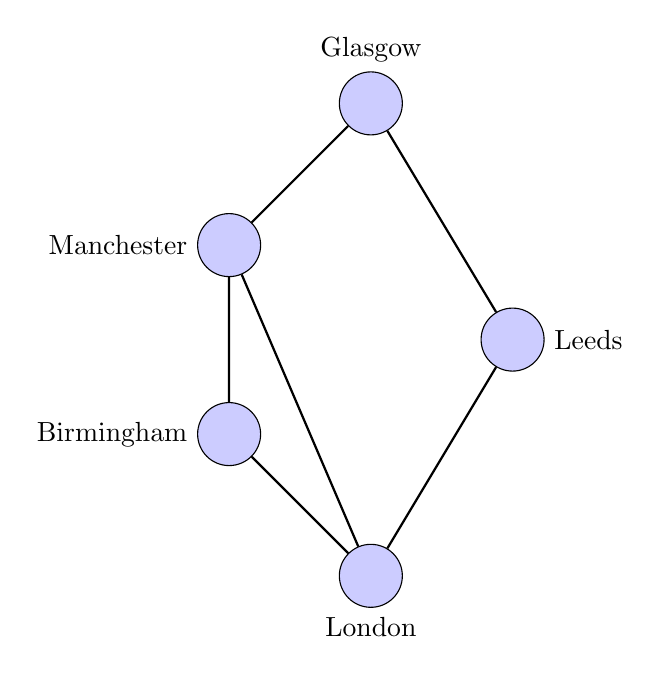
\begin{tikzpicture}[scale=1.2]
    % Define node positions (clockwise from bottom)
    \node[circle, draw, fill=blue!20, minimum size=0.8cm, label=below:London] (London) at (0, -2) {};
    \node[circle, draw, fill=blue!20, minimum size=0.8cm, label=left:Birmingham] (Birmingham) at (-1.5, -0.5) {};
    \node[circle, draw, fill=blue!20, minimum size=0.8cm, label=left:Manchester] (Manchester) at (-1.5, 1.5) {};
    \node[circle, draw, fill=blue!20, minimum size=0.8cm, label=above:Glasgow] (Glasgow) at (0, 3) {};
    \node[circle, draw, fill=blue!20, minimum size=0.8cm, label=right:Leeds] (Leeds) at (1.5, 0.5) {};
    
    % Draw edges
    \draw[thick] (London) -- (Birmingham);
    \draw[thick] (London) -- (Leeds);
    \draw[thick] (London) -- (Manchester);
    \draw[thick] (Birmingham) -- (Manchester);
    \draw[thick] (Manchester) -- (Glasgow);
    \draw[thick] (Glasgow) -- (Leeds);
\end{tikzpicture}
\caption{Network 2}
\end{subfigure}
\caption{Comparison of two network topologies with 5 UK cities.}
\label{fig:networks}
\end{figure}

\section{Methodology}
\subsection{Routing}
The first step was to determine the proportion of capacity that should be allocated to each route joining two nodes in the network. The number of channels available to each link is approximately 
\begin{equation}
N_i = N_{busiest} \times \frac{C_i}{C_{busiest}}
\label{eq:num_channels}
\end{equation}
where \(N\) is the number of channels and \(C\) is the capacity of a link. Hence an optimal routing maximised the total channels (and thus total capacity) by minimising the usage of the busiest link. This was framed as the multi-commodity flow problem and solved with linear programming given the demands between nodes and the maximum capacities of each link. The result was the relative usage of every route through the network.
\subsection{Channel Assignment}
Equation \ref{eq:num_channels} indicates that the maximum number of channels should be assigned to the busiest link. Here the EDFA limits this to 25. Channels were then assigned to each route passing through the busiest link in proportion to their usages. One of these routes was then used as a reference to assign channels to those not passing through the busiest link as
\begin{equation}
N_i = N_{ref} \times \frac{C_i}{C_{ref}}.
\end{equation}
A final check was then performed to ensure every link had at most 25 channels.
\subsection{Calculating NSR of a Link}
The NSR in decibels over an integer number of spans is given by
\begin{equation}
    NSR_{dB} = NF + 10 \log_{10}(N_s) + \alpha L_s + 10 \log_{10}(R_sh\nu \times 10^3) - P_{TX,dBm} + 10 \log_{10}(1.5)
    \label{eq:nsr_spans}
\end{equation}
where \(NF\) is the noise figure of the EDFA, \(N_s\) is the number of spans, \(\alpha\) is the fiber attenuation in dB/km, \(L_s\) is the span length in km, \(R_s\) is the symbol rate, and \(P_{TX, dBm}\) is the transmitted power in dBm. The final term is due to non-linear noise being half that of amplifier noise at the optimum launch power. This assumed a brick-wall shaped pulse and that the amplifier gain in dB is \(\alpha L_s\). In practice the link length was not always an integer number of spans, so the additional NSR of the remaining length had to be included. The NSR due to non-linear effects in the excess fiber is given by
\begin{equation}
    NSR_{add} = \frac{N_{NLI}}{G_{TX}} = C_{NLI} G_{TX}^2
\end{equation}
where \(C_{NLI}\) is the non-linear coefficient of the excess fiber and \(G_{TX}\) is the PSD of the signal at the start of the excess fiber. An additional amplifier may be needed at the end of the link, in which case the NSR is further increased by
\begin{equation}
    NSR_{amp} = \frac{N_{ASE}}{(10^\frac{-\alpha L_x}{10}g) \times G_{TX}}
\end{equation}
where \(N_{ASE}\) is the PSD of the amplifier noise, \(L_x\) is the excess length in km and \(g\) is the linear amplifier gain.

\subsection{Determining Amplifier Gain and Span Length}
The amplifiers used had an unsaturated gain \(G_0\) of 25 dB and a total saturation output power across all channels \(P_{sat, dBm}^{out}\) of 23 dBm. The true gain of the amplifier in dB is
\begin{equation}
    G = G_0 - 10 \log_{10} (1 + \frac{P_{out}}{P_{sat}})
    \label{eq:gain}
\end{equation}
where \(P_{out}\) is the total output power across all channels in mW, and \(P_{sat} = \frac{1}{\ln 2} P_{sat}^{out}\) in mW. Equation \ref{eq:nsr_spans} is valid for the optimum launch power over one channel \(P_{TX, opt} = R_s\sqrt[3]{\frac{N_{ASE}}{C_{NLI}}}\). This was computed iteratively by first assuming \(G = G_0\) to find an initial value of the optimum launch power, then using this to find the total power over all channels and updating \(G\) with Equation \ref{eq:gain}. This was done until the gain and optimum launch power converged. The resulting span length \(L_s = \frac{G}{\alpha}\) was then computed for each link.
\subsection{Calculating NSR of a Route}
The total NSR along a route was the sum of the NSRs of each link it passed through and the NSRs of any additional amplifiers. To ensure the optimum power is used at the start of every link, an amplifier was added between links \(i\) and \(i+1\) with linear gain \(g = \frac{P_{RX, i}}{P_{TX, i+1}}\) where \(P_{RX,i}\) is the received power at the end of the link \(i\) including the loss of the additional fiber that is a fraction of the span length and \(P_{TX, i+1}\) is the optimum launch power of the next link. [FIX THIS!!!] 
\subsection{Validating a Route}
A route in the network was valid for a given transceiver mode if it could deliver an output power greater than the minimum of the transceiver and an NSR lower than the maximum of the transceiver. Fiber type was kept the same throughout the network but the transceiver mode could vary between routes as they operated on individual channels. For each fiber type, the NSR and output power of every route was calculated then checked against the transceiver constraints. The transceiver mode that had the highest data rate and was valid for the route \(D_{\max}\) was then used to find the capacity of a route \(C_r = N_rD_{\max}\), where \(N_r\) is the number of channels assigned to the route.
\subsection{Optimization and Measuring Resilience}
The total capacity of a network was found by summing the capacities of every route. This was repeated over all fiber types to find the highest capacity and thus the optimal design for each network. Resilience was measured by finding the lowest capacity when any pair of links (both directions) was broken and the corresponding drop in capacity to every city.


\section{Results}


\end{document}